\documentclass[12pt]{report}
\usepackage{amssymb}
\usepackage{multicol}
\usepackage{graphicx}
\usepackage{subfigure}
\usepackage{verbatim}
\usepackage[letterpaper,left=1cm,right=2cm, top=1.5cm,
bottom=1.5cm,head=0cm,foot=1cm]{geometry}

\parindent=0in


\newcommand{\m}{\mbox{ m }}
\newcommand{\kg}{\mbox{ kg }}
\newcommand{\s}{\mbox{ s }}
\newcommand{\ke}{\mbox{\small KE}}
\newcommand{\pe}{\mbox{\small PE}}


\newcommand{ \probDir}[1]{{ \bf\small #1 \mbox{  }}}
\newcommand{ \multChoice}[5]{ \item #1 \begin{multicols}{2} \begin{enumerate} \item #2 \\ \item #3 \\ \item #4 \\ \item #5 \\ \end{enumerate} \end{multicols}}

\newcommand{ \breakList}{\setcounter{saveenum}{\value{enumi}} \end{enumerate}}
\newcommand{ \contList}{\begin{enumerate} \setcounter{enumi}{\value{saveenum}}}

\newcounter{saveenum}

\def \wspace{5cm}

%%%%%%%%%%%%%%%%%%%%%%%%%%%%%%%%%%%%%%%%%
\begin{document}

{\bf{Honors Physics} \hfill {Test 4: Forces and Friction} \hfill {Mr. Kelley}} \\ \\
%%%%%%%%%%
\mbox{} \hfill $\sum F=ma$ \hfill $F_f=\mu F_\bot$ \hfill \mbox{}


\begin{enumerate}
%\multChoice{What is the answer?}{is it a?}{is it b?}{or maybe c?}{how about d?}
\item A mass of 35 kg is hanging in the center of a clothesline.
\begin{enumerate}
\item What is the force of gravity on the mass?\\
\item What is the tension in each part of the line?\\
\end{enumerate}
\vspace{1cm}

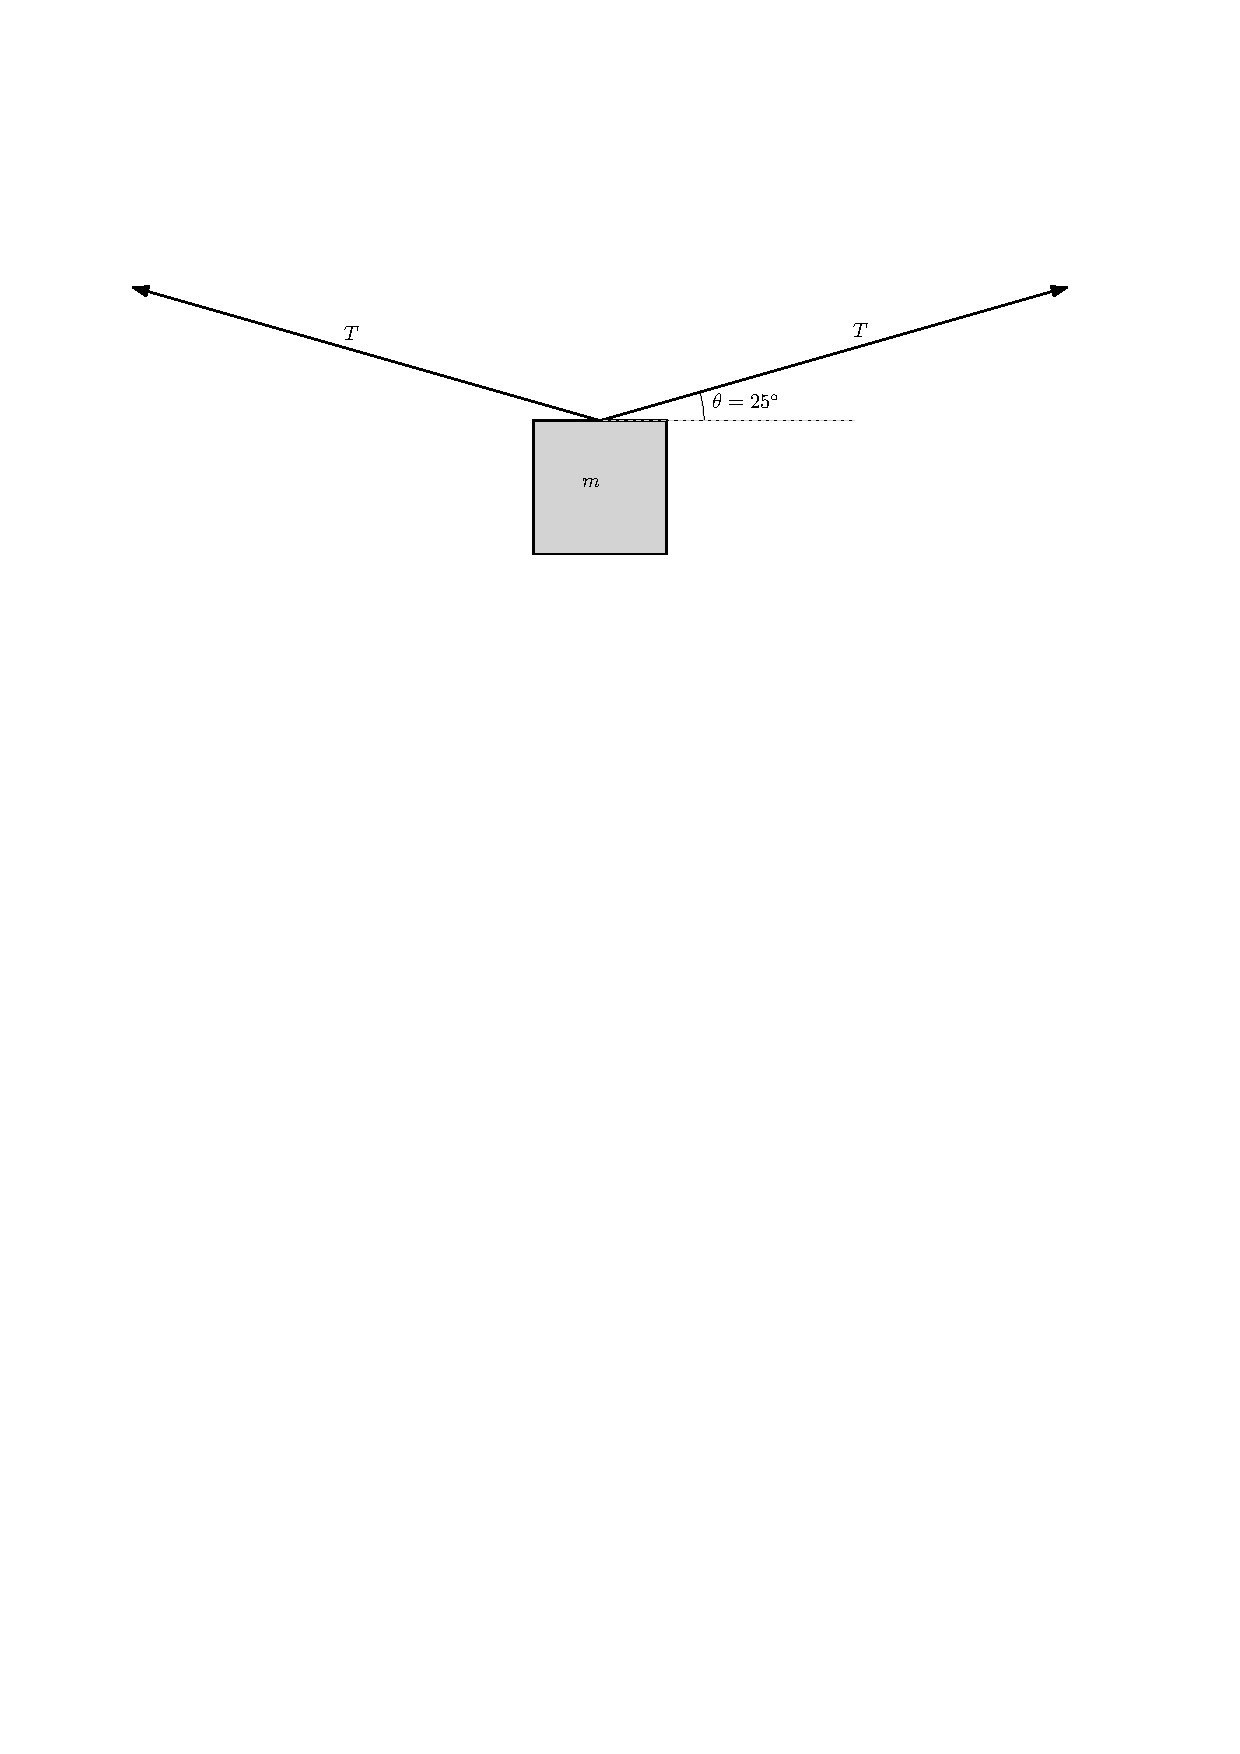
\includegraphics{massClothesline} 

\vspace{4cm}

%\item 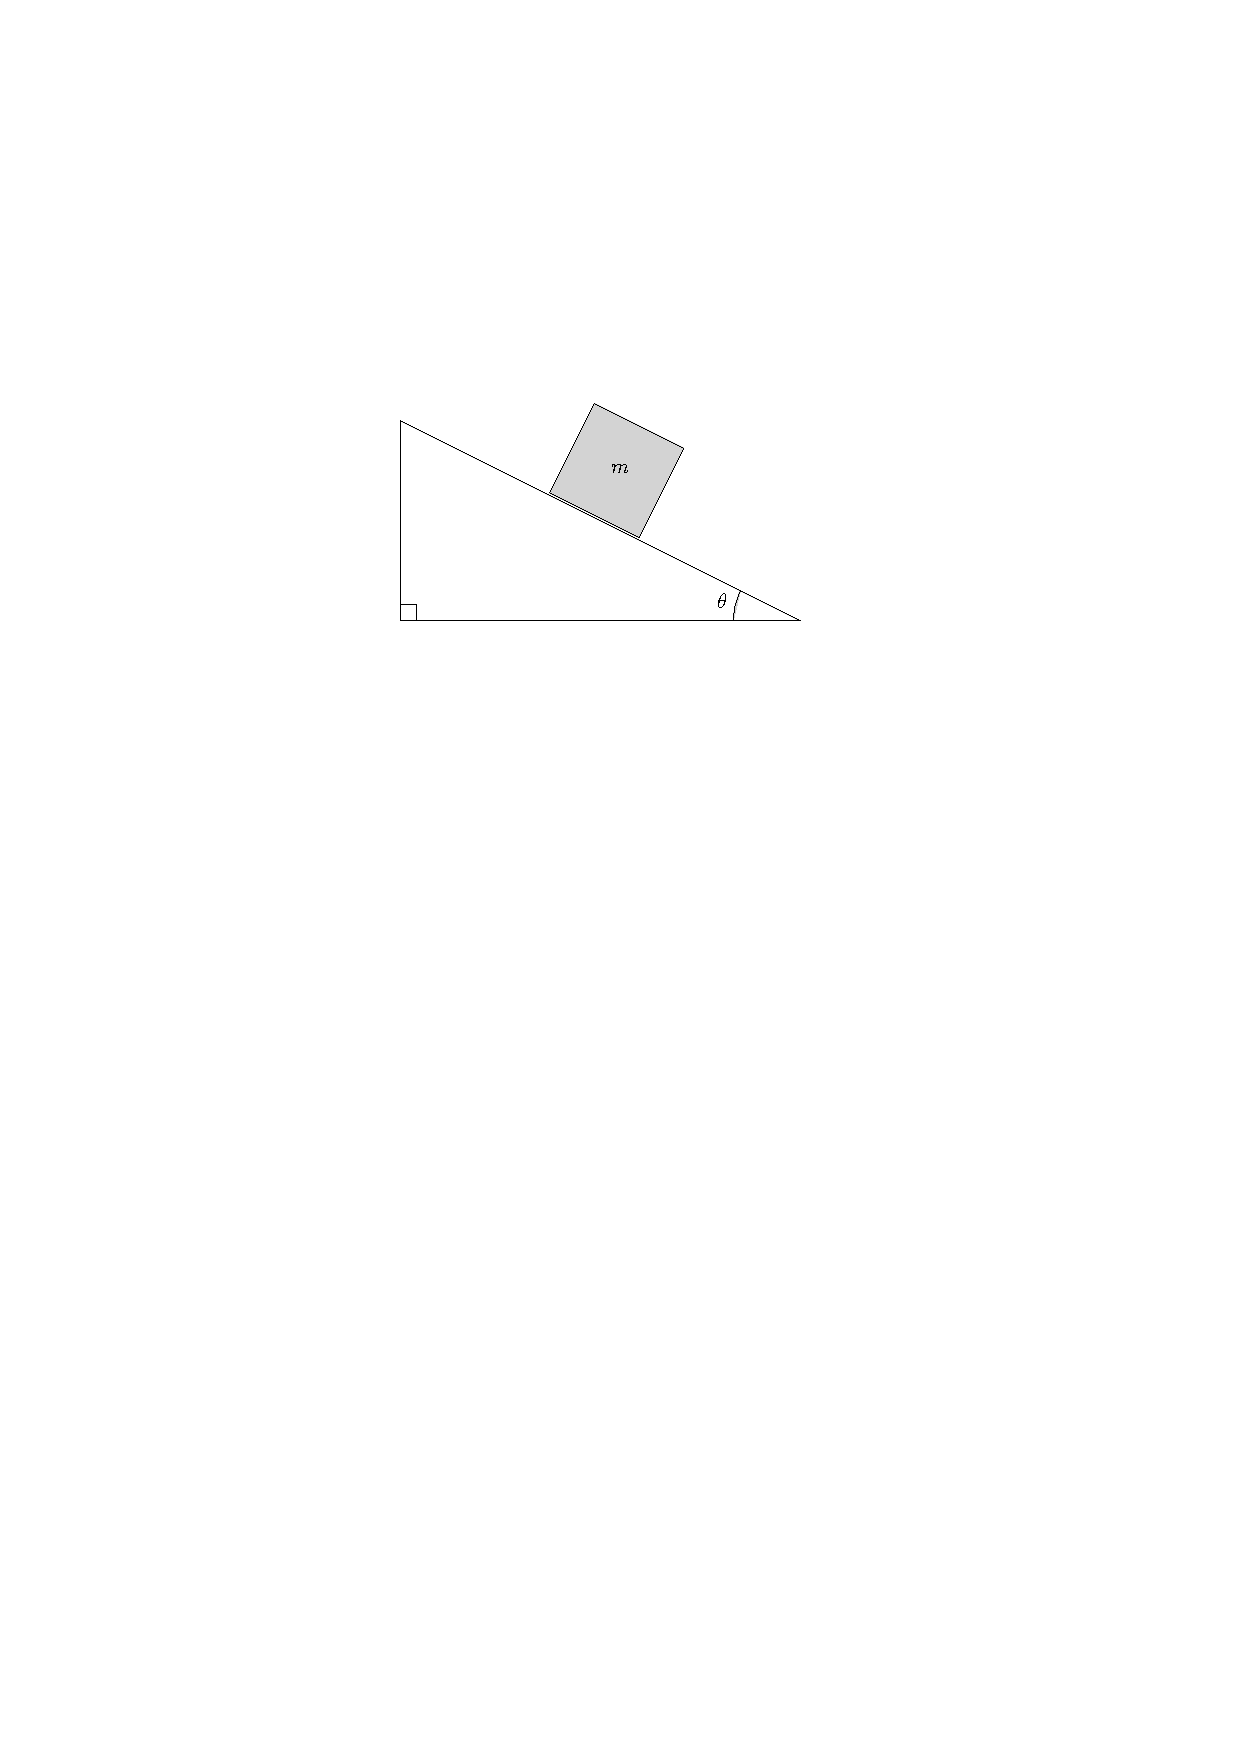
\includegraphics{inclinedPlane}

\item A mass of 22 kg slides down an plane at constant velocity.  If $\theta = 22^\circ$, what is the coefficient of friction in this system?

\vspace{1cm}

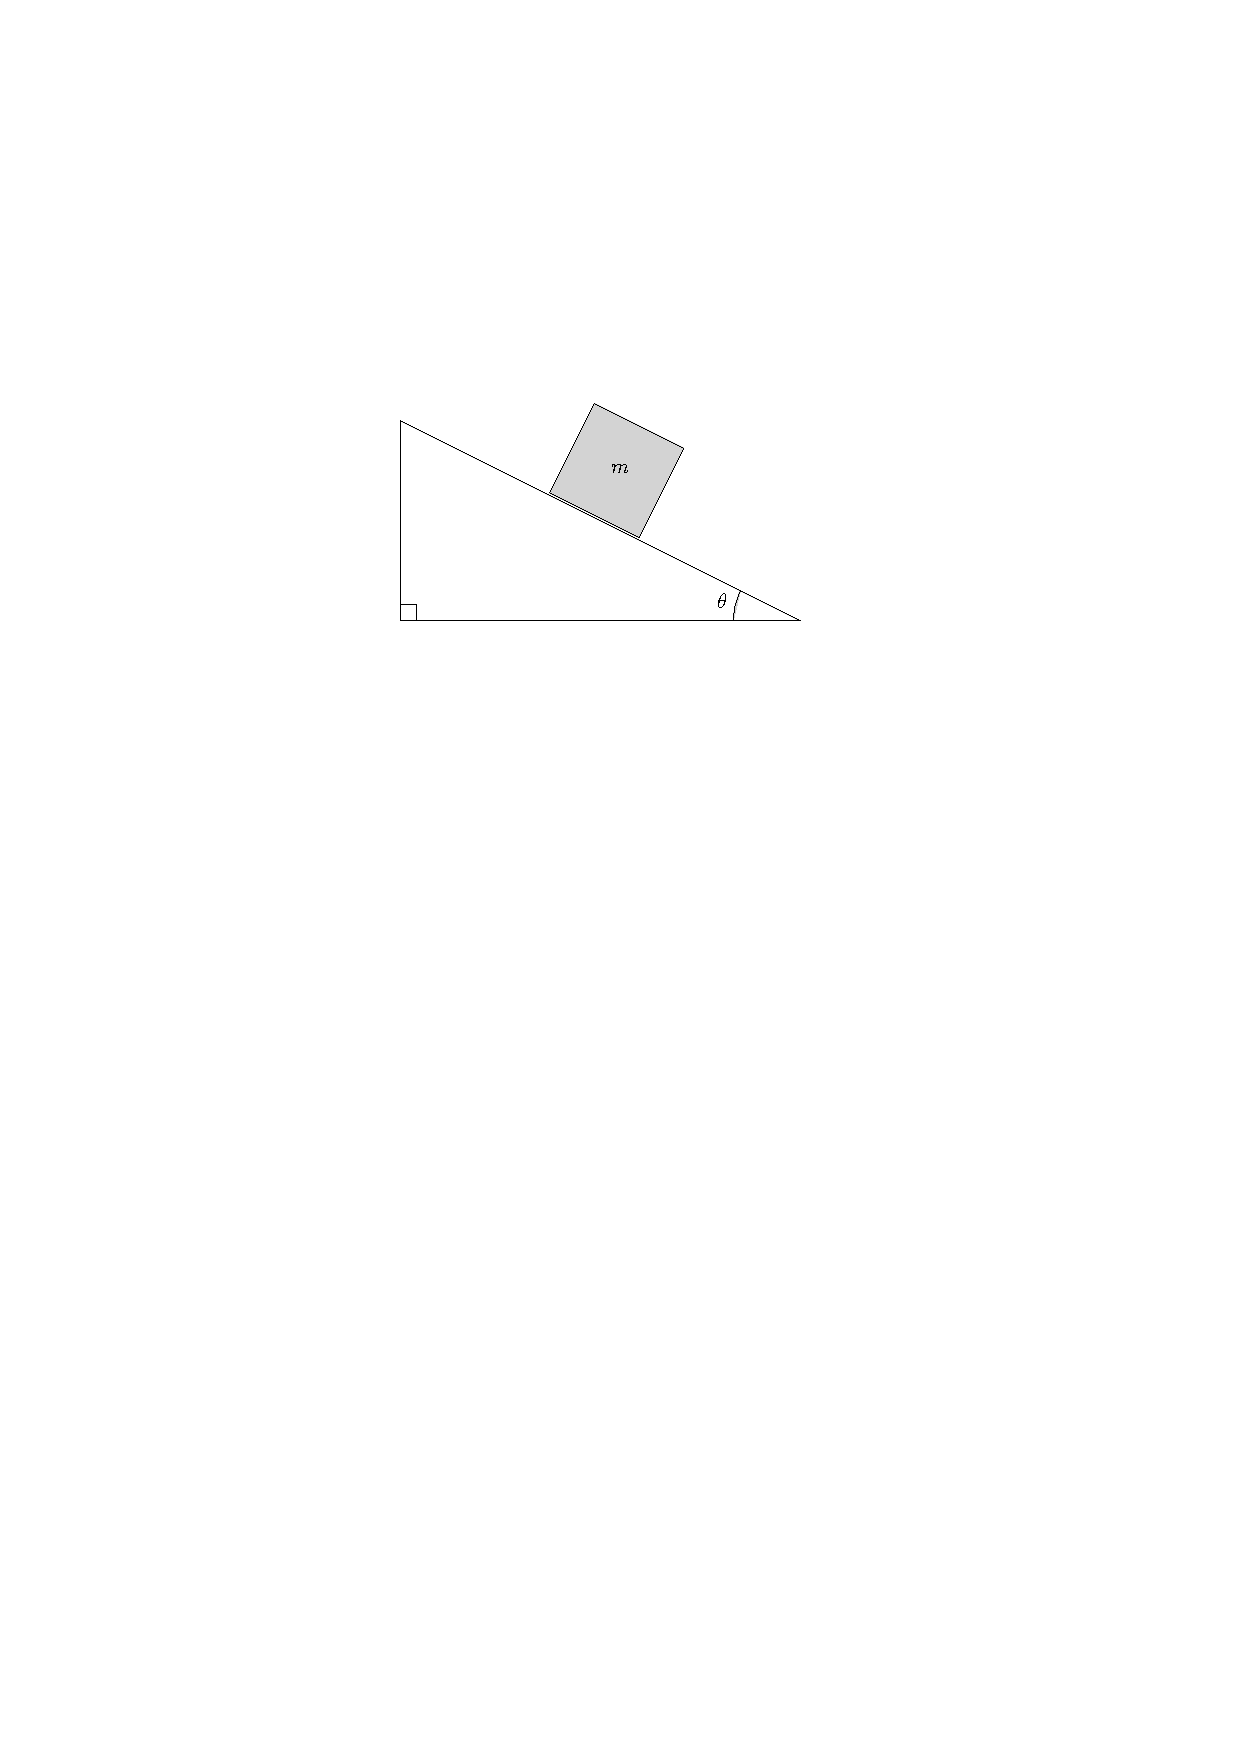
\includegraphics{inclinedPlane}

\pagebreak

%%%%%%%
\item A 5 kg mass is being dragged by a force of 24 N at an angle $\theta = 20^\circ$, and the coefficient of friction between the two surfaces is 0.30 \\
\mbox{} \hfill 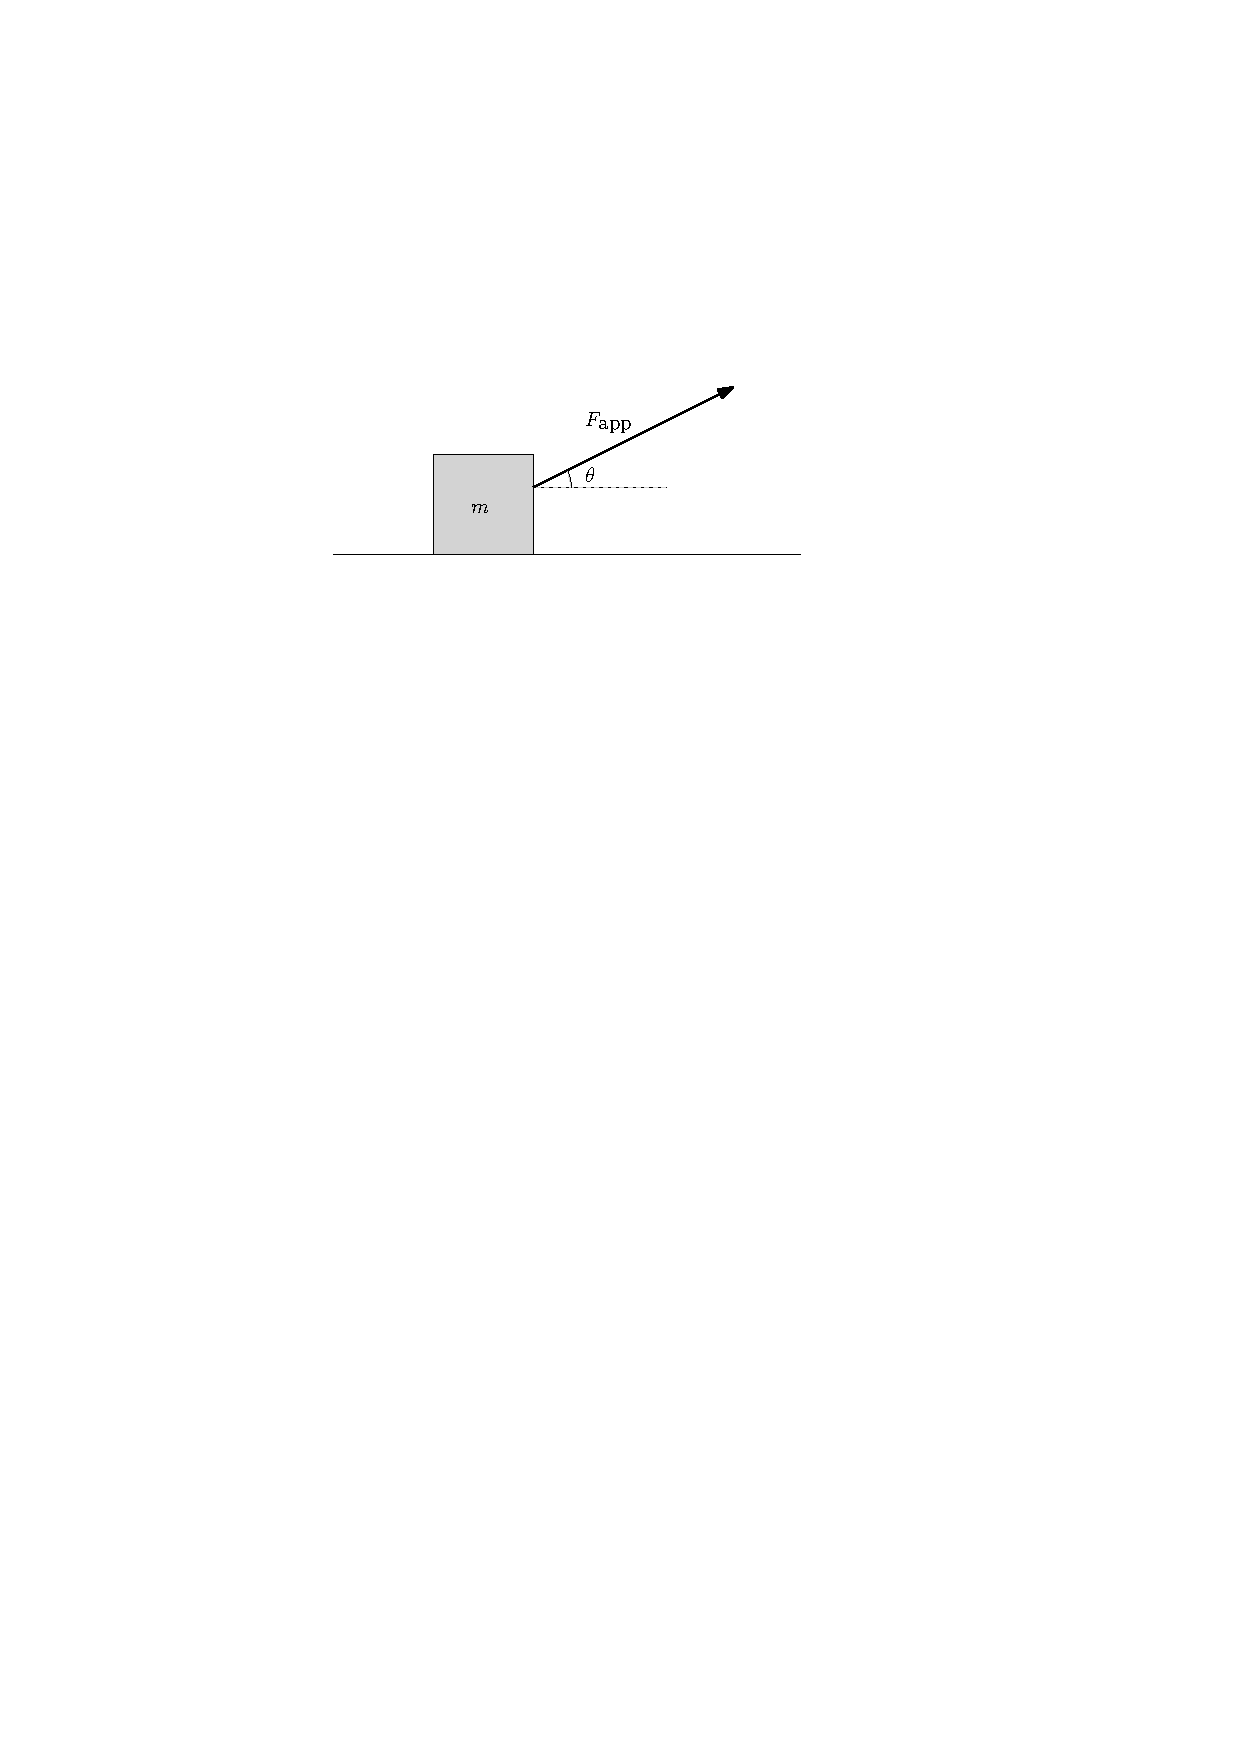
\includegraphics{boxAngle} \hfill \mbox{}
\begin{itemize}
\item What is the normal force on the mass?
\vspace{4cm}
\item What is the acceleration of the mass?
\vspace{5cm}
\end{itemize}

\item Consider the following \emph{frictionless} inclined plane and pulley system.  If $\theta = 30^\circ$ and the masses are equal, write an expression for the acceleration of the system.  Use $\sin \theta = \frac{1}{2}$ and $\cos \theta = \frac{\sqrt{3}}{2}$.

\vspace{1cm}

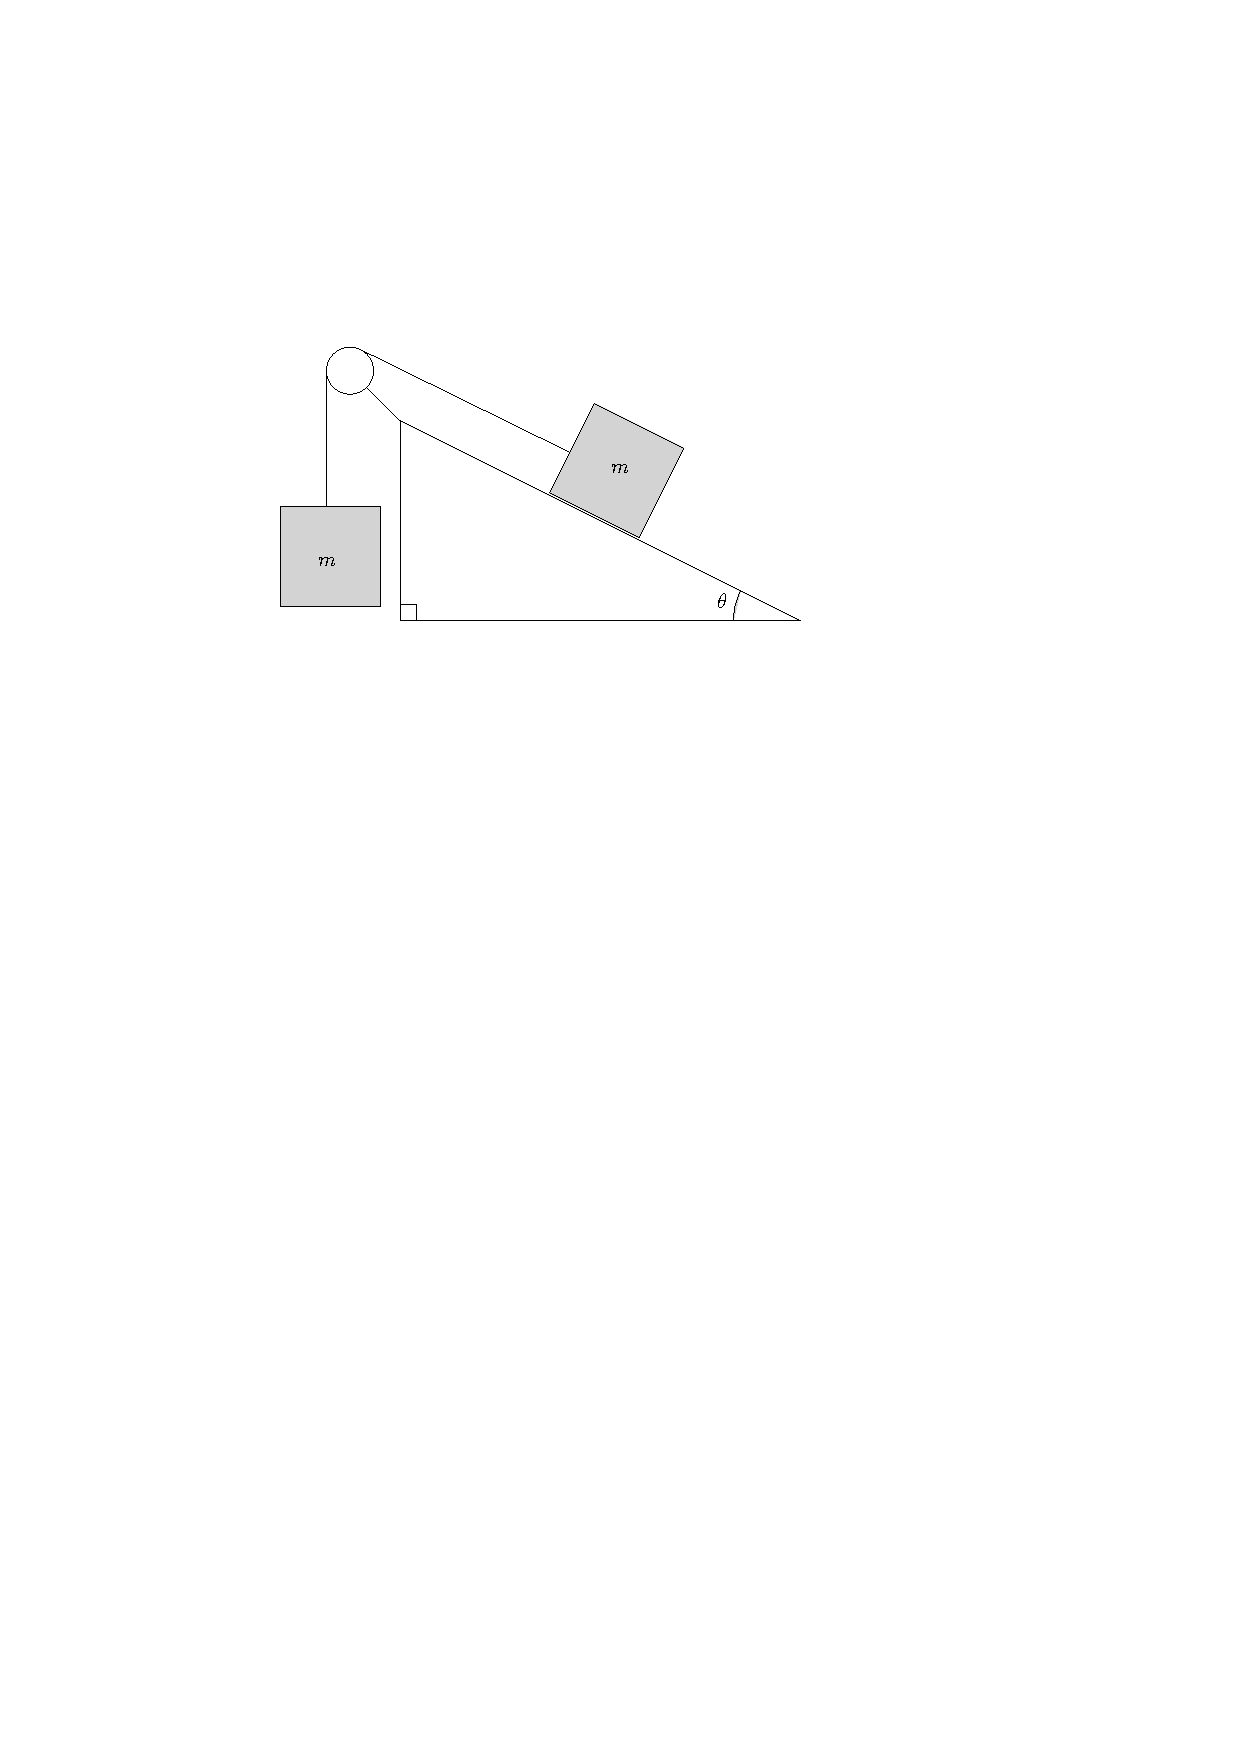
\includegraphics{inclinedPulley} \\

\pagebreak

\item Suppose $m = 15$ kg and the coefficient of friction in this system is 0.30  \\

\vspace{1cm}
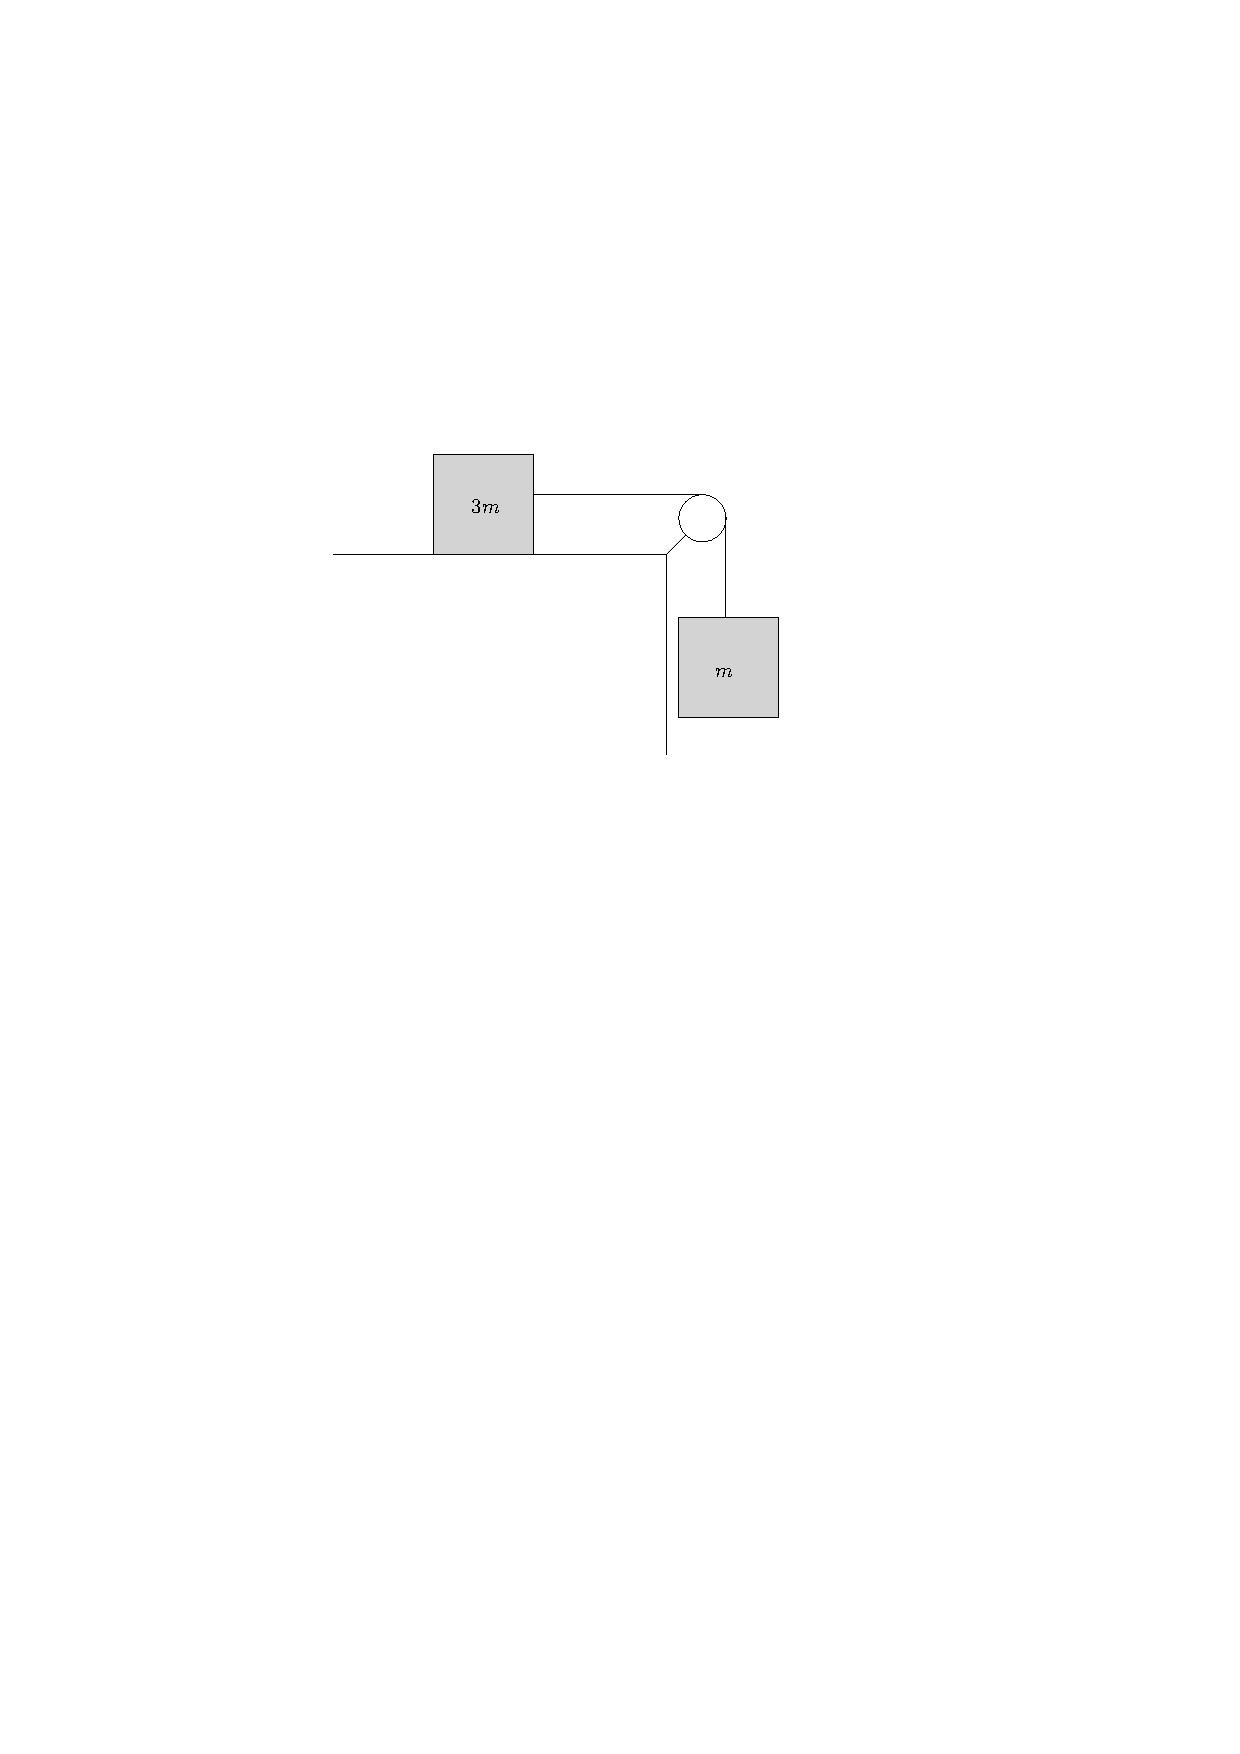
\includegraphics{flatMassPulley2}
\vspace{2cm}
\begin{enumerate}
\item What is the acceleration of the boxes? \\

\item What if the coefficient of friction is 0.40?
\end{enumerate}

\pagebreak

\item A motorcyclist is exiting the freeway.  She has measured the $\Delta y$ and $\Delta x$ of the off-ramp previously (see diagram).  She wants to calculate how much friction is inherent in her bike system.  At the top of the ramp she is traveling at 65 mph, she then \emph{coasts} to the bottom (without using the gas or brakes) where she is traveling at 40 mph.  The bike and the motorcyclist together weigh 182 kg.  Demonstrate the calculation she has to make to find $\mu$ of her bike. \\  (Hint: start with $v_f^2 = v_\circ^2 + 2a \Delta x$, and 1 mile = 1609 meters) \\

\vspace{1cm}

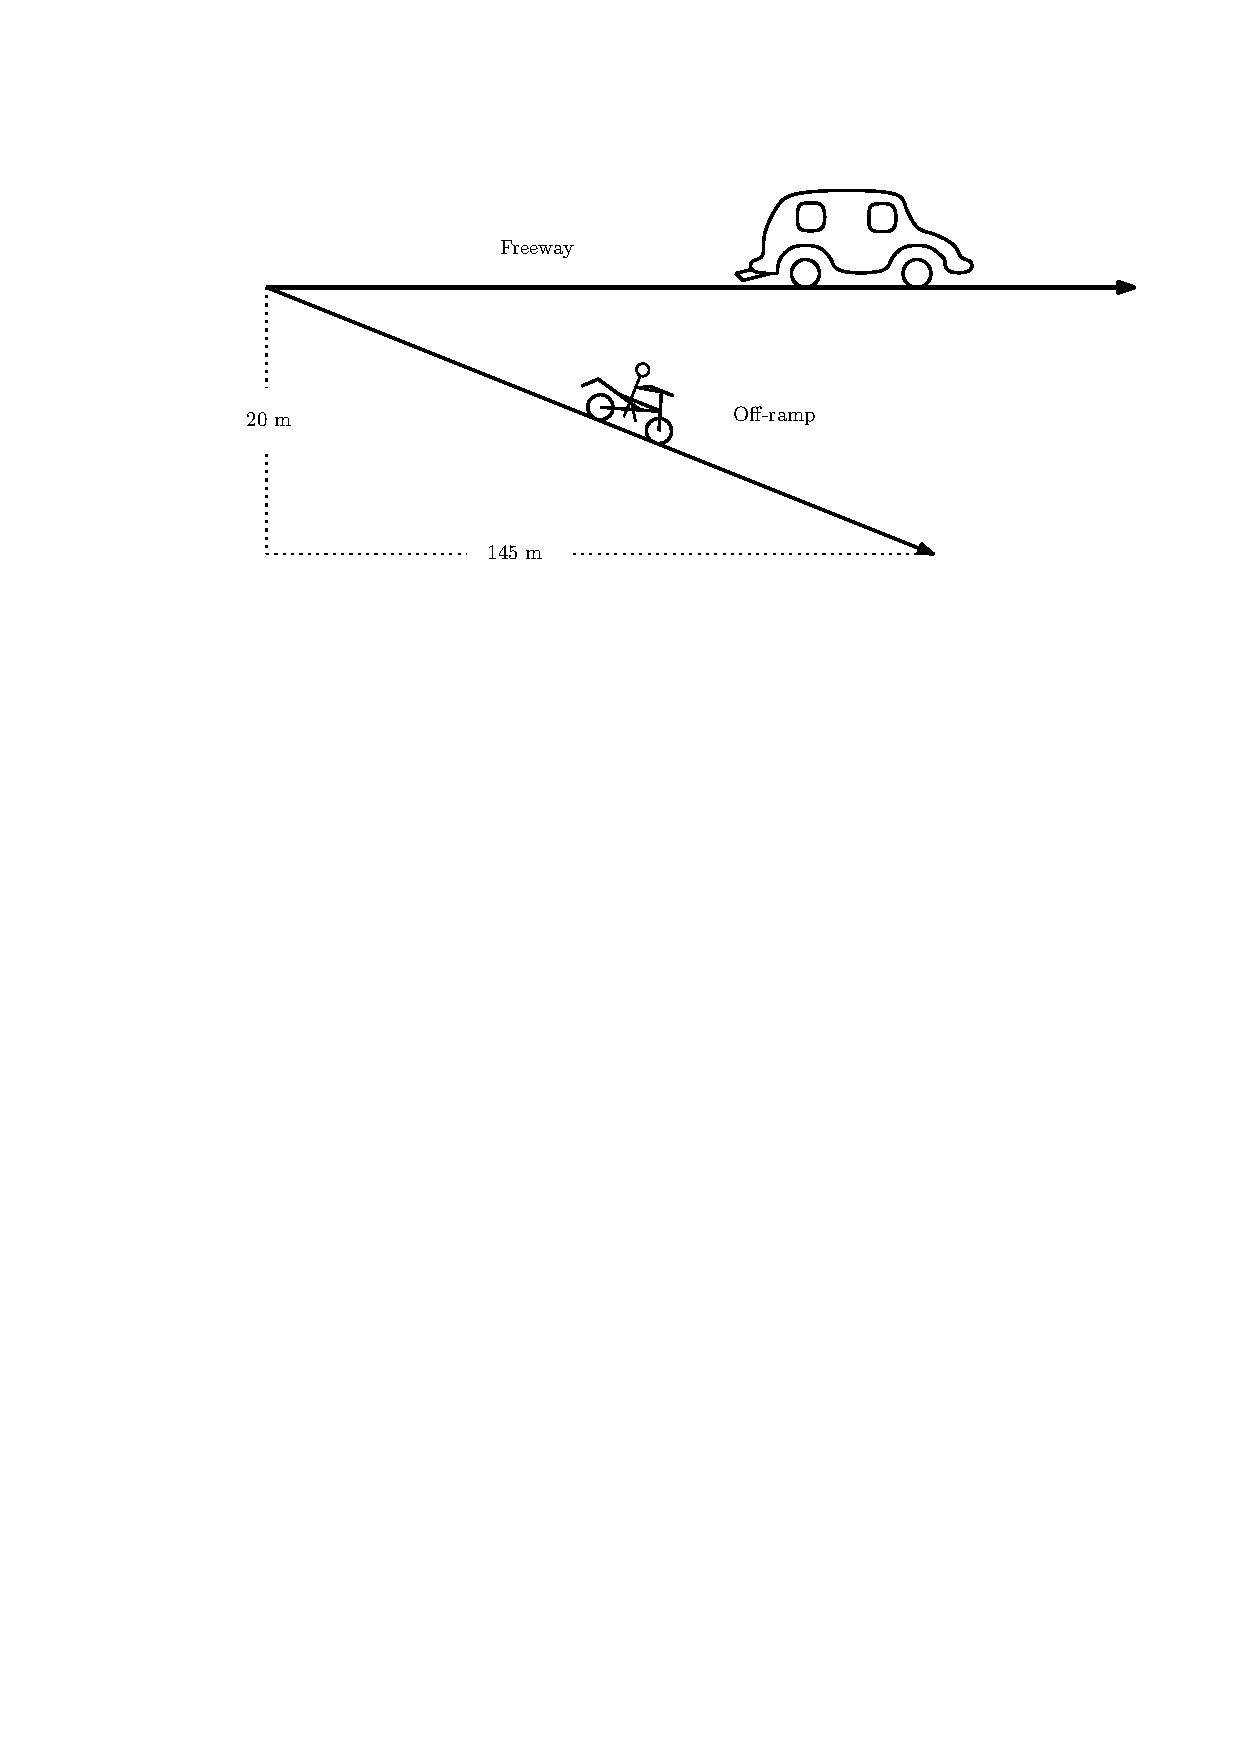
\includegraphics{motorcyclist}


\vfill
%%%%
\end{enumerate}




\end{document}